\newcommand{\pdftitel}{Cimarron Herget 2017}
\newcommand{\autor}{Marius Herget}
\newcommand{\version}{draft} % change to "final" to disable comments | "draft" shows notes/tbds/etc
\newcommand{\isPrintVersion}{true}

\documentclass[%
	pdftex,
	oneside,        % Einseitiger Druck.
	12pt,           % Schriftgroesse
	parskip=half,   % Halbe Zeile Abstand zwischen Absätzen.
	headsepline,    % Linie nach Kopfzeile.
	footsepline,    % Linie vor Fusszeile.
	english,        % Translator
]{article}


\usepackage[utf8]{inputenc}
\usepackage[english]{babel}
\usepackage[english]{isodate}
\usepackage[parfill]{parskip}

\usepackage[inline]{enumitem}


\usepackage{ltablex} % mix out of tabularx and longtable
\usepackage{multirow}

\usepackage{graphicx}
\usepackage{wrapfig}
\usepackage{subcaption} %To create subfigures
% \usepackage{subfig} %To create subfigures
\usepackage{placeins} % FloatBarrier
\usepackage{floatrow}
\graphicspath{ {./images/} }

\usepackage[]{geometry}
\usepackage{pdflscape}
\usepackage{booktabs}

\usepackage[most]{tcolorbox}
\usepackage{cleveref}
\usepackage{tikz}
\usetikzlibrary{decorations.pathreplacing,shapes,arrows,positioning}
\usetikzlibrary{positioning}
\usetikzlibrary{backgrounds}
\usetikzlibrary{patterns}

\tikzstyle{input} = [coordinate]
\tikzstyle{output} = [coordinate]
\tikzstyle{block} = [rectangle, draw, text width=5em, text centered,  minimum height=4em]
\tikzstyle{storage} = [cylinder, shape border rotate=90, aspect=0.25, draw]
\tikzstyle{label} = [text width=2.4cm, text centered]
\tikzstyle{wideblock} = [rectangle, draw, text width=7em, text centered,  minimum height=4em]

\usepackage[absolute]{textpos}
\setlength{\TPVertModule}{1mm}
\setlength{\TPHorizModule}{1mm}
\usepackage[\version, layout={inline,index}, singleuser]{fixme}
% Side characters
\newcommand{\impmark}{\strut\vadjust{\domark}}
\newcommand{\domark}{%
	\vbox to 0pt{
		\kern-\dp\strutbox
		\smash{\llap{*\kern1em}}
		\vss
	}%
}
\newcommand{\impquest}{\strut\vadjust{\doquest}}
\newcommand{\doquest}{%
	\vbox to 0pt{
		\kern-\dp\strutbox
		\smash{\llap{?\kern2em}}
		\vss
	}%
}
% Fixme
\fxsetup{envlayout=plain}

\usepackage[backend=bibtex,style=numeric]{biblatex}
\addbibresource{lib/research.bib}


\begin{document}
% TBD
\newcommand{\tbd}[1][null]{
    \ifthenelse{\equal{#1}{null}}
    {\ignorespaces\textit{\impmark\color{orange}\textbf{TBD}}}
    {\ignorespaces\textit{\impmark\color{orange}[TBD: #1]}}
}
\newcommand{\todo}[1][null]{
    \ifthenelse{\equal{#1}{null}}
    {\ignorespaces\textit{\impmark\color{orange}\textbf{TBD}}}
    {\ignorespaces\textit{\impmark\color{orange}[TBD: #1]}}
}



% \maketitle\tableofcontents\newpage
\pagenumbering{Roman}
\title{\textbf{Cimarron}\\Stabilisation of videos in modern \texttt{C++}}
\date{\today}
\author{    Marius Herget\\[2em]
            % {\small Practical Course}\\
            % \textbf{Advanced Software Development with Modern \texttt{C++}}\\
            \textit{in partnership with}\\[2em]
            \textit{Institute for Computer Science}\\
            \textit{Ludwig-Maximilians-Universit\"at M\"unchen}\\[3em]
            
\includegraphics[scale=0.5]{lmu-siegel}}
% (feature abused for this document to repeat the title also on left hand pages)
\maketitle
\newpage
% \tableofcontents
% \newpage
% \listoffigures
% \newpage
% \listoftables
\pagenumbering{arabic}

\section{Idea}
Video stabilization is used ever since cameras evolved. In the early days physicial stabilization techniques as tripods were used. In the following centuries cameras enhanced step by step. New solid and dynamic methods were invented like steady cams, dollys, shoulder rigs and many more. With the invention of digital photography and videos another possible solutionwas found: digital image stabilization. Different techniques like optical flow analysis or warp stabilization were developed. \texttt{Cimarron} implements such a feature tracking method for motion compensation.

\section{Theoratical introduction}\label{sec:thintro}
New technologies emerge each year. In the last years espacially phones and small cameras were published. Under ideal condition recent smartphone's cameras pictures cannot be distinguished from professional cameras anymore. Nevertheless, a smartphone video is often detectable by its \textit{handheld}, shaky look. As already mentioned within the short introduction different methods can be used to compensate this motion.

The general idea of video stabilization is to counter, smoothen or to minimize unwanted shakes. In general video motion stabilization can be classified in three categories: mechanical based, optical based and electronical based. Instead of using specific hardware like the first two methods, the electronical approach uses computing power to implement image processing techniques in the  postproduction step. \cite{blockTang}

In order to compensate the unwanted movement of the camera, motion can be described in various forms. \textit{Translation} is the simplest form of expression. In this concept direct, linear movement of a single point is described as the distance it covered within a certain time. This can enhanced with the combination of \textit{rotational motion}.  In comparision to translational movement it specifies the angle a point / body covers in a given timeframe. Examples can be seen in \cref{fig:motionmodels}.
\begin{figure}[h!]\centering
    \begin{minipage}{.45\textwidth}\centering
        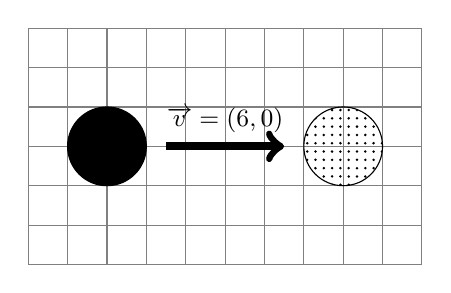
\begin{tikzpicture}[scale=1]
        \draw[step=0.5cm,gray,thin] (-3,-2) grid (2,1);
        \draw[black, fill = black] (-2,-0.5) circle [radius=.5];
        \draw[black, pattern=dots] (1,-0.5) circle [radius=.5];
        \draw[thick, black, ->, line width=1mm] (-1.25,-0.5) -- node[above]{\small$\overrightarrow{v} = (6,0)$} (0.25,-0.5);
        \end{tikzpicture}
        \subcaption{Translational motion}
    \end{minipage}
    \begin{minipage}{.45\textwidth}\centering
        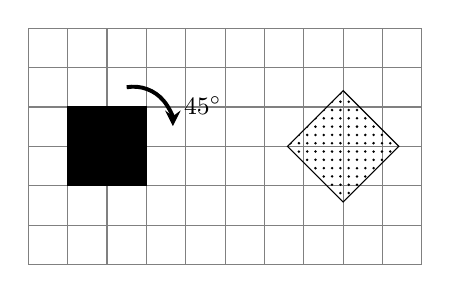
\begin{tikzpicture}[scale=1]
        \draw[step=0.5cm,gray,thin] (-3,-2) grid (2,1);

        \draw[black, fill = black]  (-2.5,0) rectangle (-1.5,-1);
        \draw[black, pattern=dots,rotate around={45:(1,-0.5)}] (0.5,0) rectangle (1.5,-1);
        % \draw[thick, black, ->, line width=1mm] (-1.25,-0.5) -- (0.15,-0.5);
        \draw[-stealth,  black, line width=0.5mm] (-1.75,0.25) arc  (100:0:0.5)node[above right]{\small$45^\circ$};
        \end{tikzpicture}
        \subcaption{Rotational motion}
    \end{minipage}
    \caption{Differnt motion models}
    \label{fig:motionmodels}
\end{figure}

Another motion model is \textit{perspective}. As well as translational and rotational movement it can be described as vectors and scalars. The inverse of each model can be used as the source for the stabilization.


\section{Modeling}

\section{Implementation}
\texttt{Cimarron} is implement in \texttt{C++14} and heavily depends on the \texttt{OpenCV} library.
\begin{figure}[h!]\centering
    \resizebox{0.9\textwidth}{!}{\centering%
    
\begin{figure}[h!]
% \centered\vspace{-4.5cm}\vspace{-4.5cm}
\small\centering\vspace{-0.5cm}
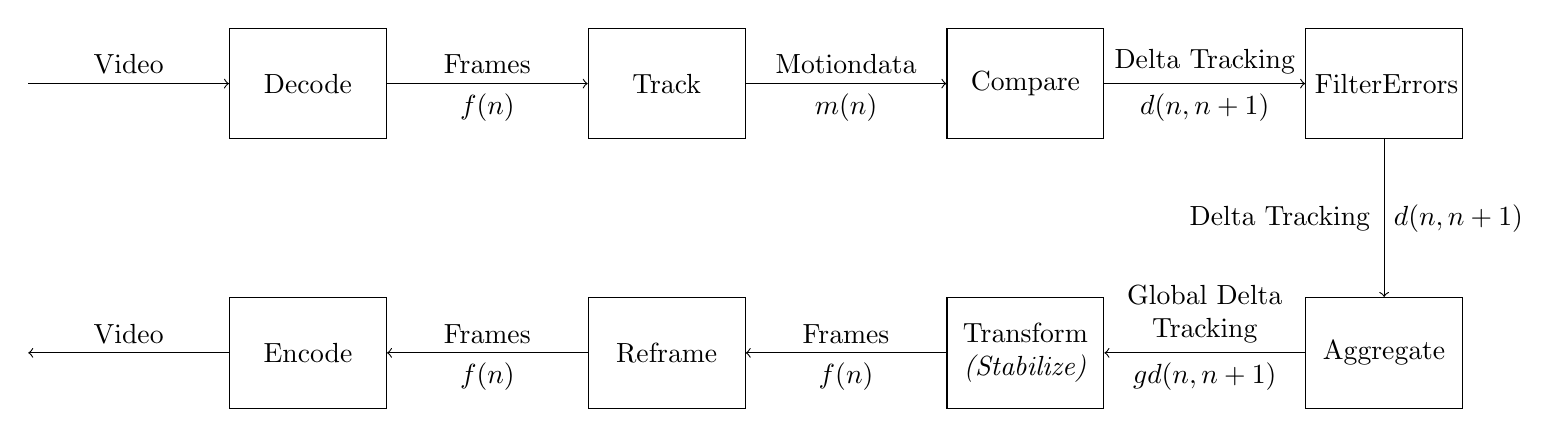
\begin{tikzpicture}[node distance=2cm and 2.55cm,auto]\centering
    \node [input, name=input] {};
    \node [block, right= of input] (pre1) {Decode};
    \node [block, right= of pre1] (analysis1) {Track};
    \node [block, right= of analysis1] (analysis2) {Compare};
    \node [block, right= of analysis2] (analysis3) {FilterErrors};
    \node [block, below= of analysis3] (analysis4) {Aggregate};
    \node [block, left= of analysis4] (stabi) {Transform \textit{(Stabilize)}};
    \node [block, left= of stabi] (post1) {Reframe};
    \node [block, left= of post1] (post2) {Encode};
    \node [input, left=of post2] (output) {t};

    % \node [storage, below right=0.5cm and 0.7cm of analysis] (analysisstorage) {DB};

     \draw[->](input) -- node {Video}(pre1);
     \draw[->](pre1) -- node[label] {Frames} node[below]{$f(n)$}(analysis1);
     \draw[->](analysis1) -- node[label]{Motiondata} node[below]{$m(n)$}(analysis2);
     \draw[->](analysis2) -- node[label]{Delta Tracking} node[below]{$d(n, n+1)$}(analysis3);
     \draw[->](analysis3) -- node[label,left]{Delta Tracking} node[right]{$d(n, n+1)$}(analysis4);
     \draw[->](analysis4) -- node[label,above]{Global Delta Tracking} node[below]{$gd(n, n+1)$}(stabi);
     \draw[->](stabi) -- node[label,above]{Frames} node[below]{$f(n)$}(post1);
     \draw[->](post1) -- node[label,above]{Frames} node[below]{$f(n)$}(post2);


     \draw[->](post2) -- node[above]{Video}(output);
\end{tikzpicture}
\caption{High-level system diagram}
\end{figure}

\tikzstyle{wideblock} = [rectangle, draw, text width=7em, text centered,  minimum height=4em]
\begin{figure}\centering\vspace{-4.5cm}
    \tcbox[enhanced, sharp corners, boxsep=1mm, boxrule=1mm,colframe=gray!10!white,
        colback=white,
        borderline={2pt}{-1pt}{gray,dotted}]
        {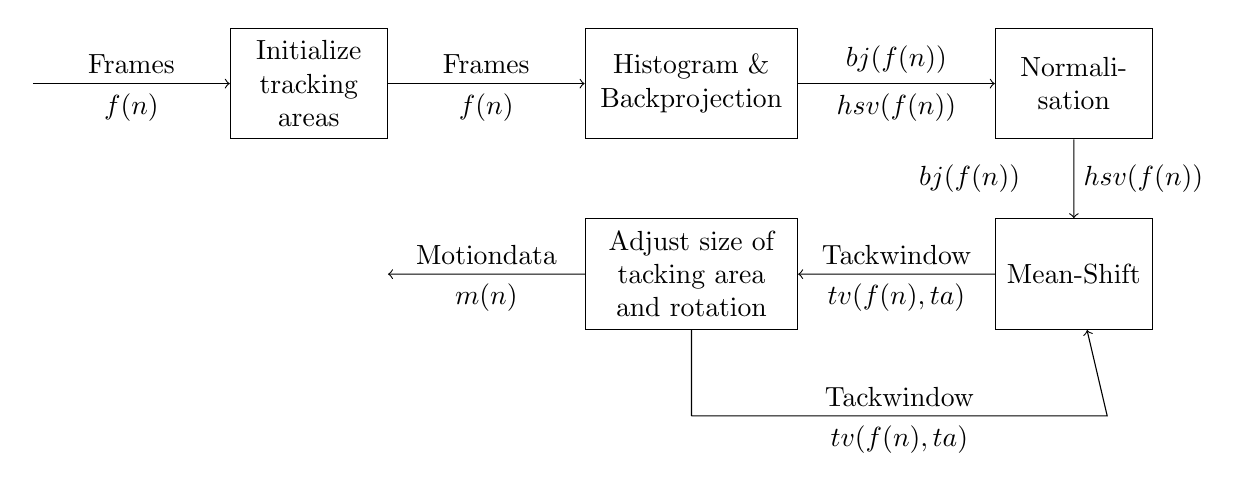
\begin{tikzpicture}[scale=0.6,node distance=1cm and 2.5cm,auto]
            \node [input, name=input] {};
            \node [block, right= of input] (pre1) {Initialize tracking areas};
            \node [wideblock, right= of pre1] (pre2) {Histogram \& Backprojection};
            \node [block, right= of pre2] (pre3) {Normali-sation};
            \node [block, below= of pre3] (pre4) {Mean-Shift};
            \node [wideblock, left= of pre4] (pre5) {Adjust size of tacking area and rotation};
            \node [input, left=of pre5] (output) {t};

            \draw[->](input) -- node[label]{Frames}node[below]{$f(n)$}(pre1);
            \draw[->](pre1) -- node[label]{Frames}node[below]{$f(n)$}(pre2);


            \draw[->](pre2) -- node[label]{$bj(f(n))$}node[below]{$hsv(f(n))$}(pre3);

            \draw[->](pre3) -- node[label, left]{$bj(f(n))$}node[right]{$hsv(f(n))$}(pre4);


            \draw[->](pre4) -- node[label, above]{Tackwindow}node[below]{$tv(f(n), ta)$}(pre5);
            \draw[->](pre5)  |- ++(0,-3cm) --node[label, above]{Tackwindow}node[below]{$tv(f(n), ta)$} ++(8.8cm,0) -- (pre4);


            \draw[->](pre5) -- node[label, above]{Motiondata}node[below]{$m(n)$}(output);
        \end{tikzpicture}
        }
    \caption{Track: CamShift algorithms}
    \label{fig:motionmodels}
\end{figure}

    \caption{High-level system diagram}
    \label{sd}}
\end{figure}
\Cref{sd} shows the general structure of the application. The differend modules each describe a specific step to achieve a smooth video. The first step is to decode the input video and to extract each frame. Therefore, it uses the \textit{frame} concept described earlier. \textit{Track} is the implementation of the OpenCV Continuously Adaptive Meanshift (CAMshift) algorithm, which is an improved version of the \textit{Meanshift} algorithm. It generates \texttt{motionData} of the tracked objects which are then compared, filtered and aggregated to achieve one global difference vector for each frame of the video. In the end these vectors are used to transform the specific frames to compensate the shaky movement. In the end these modified frames are reframed with a simple, non dynamic mask and encoded in an \textit{avi} videofile.
\texttt{Decoding} and \texttt{Encoding} are trivial due to the use of the \texttt{video++} framework and are not discussed in this documentation. More information on these topics can be found in \cite{7115639,matt42vp0:online}.

\subsection{Feature tracking}
The general concept of \texttt{Cimarron} is to track objects within the frames and follow those throughout the frames. Therefore, the CAMshift algorithm is the best way to implement the tracking. It is based on the Meanshift algorithm, which uses the simple approach of finding the maximum density region of points in a given search window. This data can be be a pixel distribution like histogram backprojection.

Firstly, Meanshift analyses the initial search window and calculates the centroid of the data. Afterwards, it uses this centroid as the new center of the search window and repeats this process, until the center of the area and the new calculated centroid are within a margin of error.

One disadvantage of Meanshift which is adressed by CAMshift ist that the tracking area has always the same size. Therefore, it is not possible to address moving objects which change their size. CAMshift was published by Gary Bradsky in his paper "Computer Vision Face Tracking for Use in a Perceptual User Interface" in 1998 and works in the following steps:
\begin{enumerate}
    \item Apply Meanshift until it converges.
    \item Updates the size of the search window.
    \item Update the rotation of the search area.
    \item Repeat step 1. until the required accuracy is met.
\end{enumerate}

A detailed explanation with specific mathematical formulas can be found in \cite{Bradski98computervision}.

\begin{figure}[ht!]\centering
    \resizebox{0.9\textwidth}{!}{\centering%
    
    \tcbox[enhanced, sharp corners, boxsep=1mm, boxrule=1mm,colframe=gray!10!white,
        colback=white,
        borderline={2pt}{-1pt}{gray,dotted}]
        {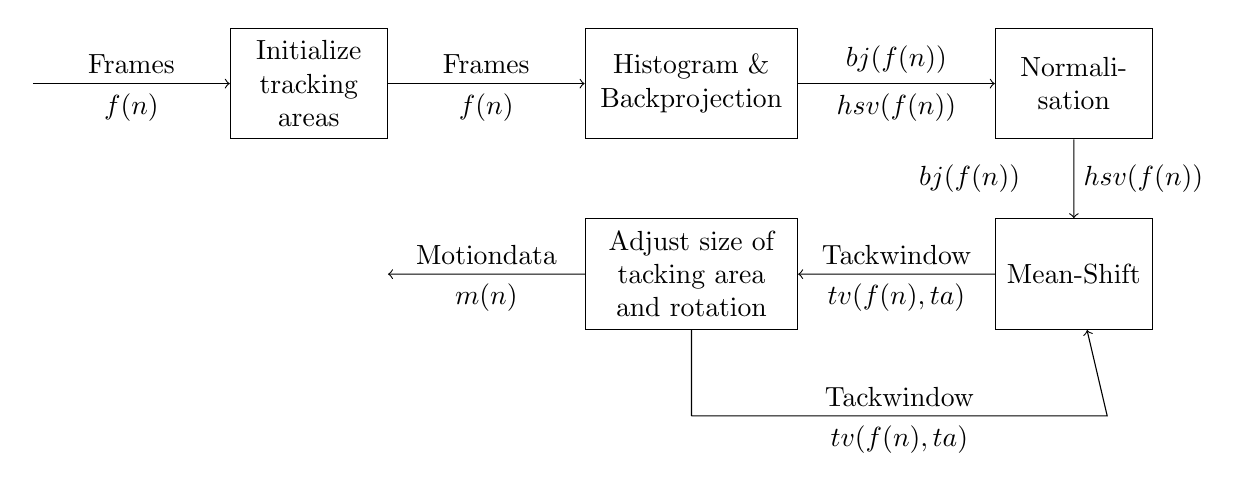
\begin{tikzpicture}[scale=0.6,node distance=1cm and 2.5cm,auto]
            \node [input, name=input] {};
            \node [block, right= of input] (pre1) {Initialize tracking areas};
            \node [wideblock, right= of pre1] (pre2) {Histogram \& Backprojection};
            \node [block, right= of pre2] (pre3) {Normali-sation};
            \node [block, below= of pre3] (pre4) {Mean-Shift};
            \node [wideblock, left= of pre4] (pre5) {Adjust size of tacking area and rotation};
            \node [input, left=of pre5] (output) {t};

            \draw[->](input) -- node[label]{Frames}node[below]{$f(n)$}(pre1);
            \draw[->](pre1) -- node[label]{Frames}node[below]{$f(n)$}(pre2);


            \draw[->](pre2) -- node[label]{$bj(f(n))$}node[below]{$hsv(f(n))$}(pre3);

            \draw[->](pre3) -- node[label, left]{$bj(f(n))$}node[right]{$hsv(f(n))$}(pre4);


            \draw[->](pre4) -- node[label, above]{Tackwindow}node[below]{$tv(f(n), ta)$}(pre5);
            \draw[->](pre5)  |- ++(0,-3cm) --node[label, above]{Tackwindow}node[below]{$tv(f(n), ta)$} ++(8.8cm,0) -- (pre4);


            \draw[->](pre5) -- node[label, above]{Motiondata}node[below]{$m(n)$}(output);
        \end{tikzpicture}
        }

    \caption{Detailed system diagram of \texttt{Track}}
    \label{sd:cam}}
\end{figure}

\Cref{sd:cam} shows the implementation of the CAMshift algorithm in \texttt{Cimarron}. The nine inital tracking areas are ordered with a $3\times 3$ Grid in the frame and can be seen as the red rectangles in \cref{fig:example:cam}. Each tracking area is indepent and uses special \texttt{camShiftTracker} class.

\begin{figure}\centering
    \includegraphics[scale=0.35]{images/tracking-example.jpg}
    \caption{Example frame: tracking}
    \label{fig:example:cam}
\end{figure}

The second step is to prepare each frame within the tracker. Therefore, a back projection is used. This methods uses the histogram of the inital tracking area in an image to show up probaibilites of colors may appear in each pixel \cite{OpenCVme45:online}. The steps of creating such this is shown in \cref{lst:prep}:
\begin{enumerate}
    \item Transform image in an color space which saves the \textit{hue} of each pixel.
    \item Extract the hue information to receive a grayscale image and normalize its histogram.
    \item Use OpenCV's \texttt{calcBackProject}.
\end{enumerate}


\begin{lstlisting}[caption={Preparation for tracking},label=lst:prep]
cv::cvtColor(image, hsv, CV_BGR2HSV);

cv::inRange(hsv, cv::Scalar(0, _smin, MIN(_vmin, _vmax)),
        cv::Scalar(180, 256, MAX(_vmin, _vmax)), mask);
int ch[] = {0, 0};
hue.create(hsv.size(), hsv.depth());
cv::mixChannels(&hsv, 1, &hue, 1, ch, 1);

if (_start) {
    cv::Mat roi(hue, _selection), maskroi(mask, _selection);
    cv::calcHist(&roi, 1, 0, maskroi, hist, 1, &_hsize, &phranges);
    cv::normalize(hist, hist, 0, 255, CV_MINMAX);
    _trackWindow = _selection;
    _start = false;
}
\end{lstlisting}

The result is an color-weighted grayscale projection of the image. \texttt{calcBackProject()} functions as follows:
\begin{enumerate*}[label= (\roman*)]
    \item Calculate weigth of each color by the histogram and
    \item Multiply each color of each pixel with its weigth
\end{enumerate*}.

From there OpenCV takes it for us by simply calling \texttt{cv::CamShift} with the created back projection, the tacking area and a terminating variable.
\begin{lstlisting}[caption={CAMshift call},label=lst:cam]
cv::CamShift(
    backproj, _trackWindow,
    cv::TermCriteria(CV_TERMCRIT_EPS | CV_TERMCRIT_ITER, 10, 1));
\end{lstlisting}

For each frame and tracking area this process is run through. The result can be seen in \cref{fig:example:cam}. The green rectangles are the tracked elements, the blue ones their bounding rectangles. Small lines indicate their movement so far through the frames.

\subsection{Movement identification of tracked objects}
The feature tracking returns a \texttt{std::vector<motionVector>} aka \texttt{motionData}. Whereby, \texttt{motionVector} is a struct of all tracking vectors in the frame and its index. This data needs to be transformed in difference vectors between frames. These results should imply how the object moved between two frames.

This is simply achieved by comparing each tracking vector by its corresponding one in the previous frame:
\[\Delta_{TrackingVector_i(m(n))} = TrackingVector_i(m(n-1)) - TrackingVector_i(m(n))\]
This results in the difference of following properties \begin{enumerate*}[label= (\roman*)]
    \item $\delta CenterPoint$, \item $\delta Angle$ and \item $\delta Area$
\end{enumerate*}. These results are combined to a frame delta data vector.

The next step is to filter tracking errors by simply looking up delta vectors which exceed a threshhold of over $10\%$ movement between two frames and deleting those.

Since the goal is to counter shaky movement by its translational and rotational movement, it is important to recognize intentional movement of objects within the frame and shakes of the camera. To achieve this, an aggregation of the delta vectors neebs to be done. The exceptions are: \begin{enumerate*}
    \item There are tracked objects in the image and \item there is only one tracked object
\end{enumerate*}. The first case returns the single delta vector as the global delta vector. The second one returns a zero vector which indicates that there is no movement between the images. The general case is that there are multiple motion vectors in each frame and therefore, multiple delta vectors.

In this case each vector is compared on time to each other vector and its similarity in translational and rotational movement is calculated.
\begin{description}
    \item[Vector similarity] is computed by the cosine similarity:
    \[cos\_sim = \frac{A \cdot B}{\Vert A\Vert \Vert B\Vert} = \frac{\sum\limits_{i=1}^{n} A_iB_i}{\sqrt{\sum\limits_{i=1}^{n}A_i^2} \sqrt{\sum\limits_{i=1}^{n}B_i^2}}\]
    It shows the the angle between two vector by calculating the dot product of each member of the vector and dividing it by the multiplication of the vector's magnitude. A result of $1$ indicates that the vectors are the same. Otherwise, a result below $0$ shows that the vectors are dissimiliar and an exact $0$ means they are orthogonal.
\begin{lstlisting}[caption={Cosine similarity},label=lst:cossim]
float dot = 0.0, denom_a = 0.0, denom_b = 0.0;

dot += A->deltaPosition.x * B->deltaPosition.x +
       A->deltaPosition.y * B->deltaPosition.y;
denom_a +=
    std::pow(A->deltaPosition.x, 2.0) *
    std::pow(A->deltaPosition.y, 2.0);
denom_b +=
    std::pow(B->deltaPosition.x, 2.0) *
    std::pow(B->deltaPosition.y, 2.0);
auto ret = dot / (std::sqrt(denom_a) * std::sqrt(denom_b));
\end{lstlisting}
    \item[Angle similarity] is simply calculated by the percantage difference between the two angles.\\
\end{description}

In the end, the analysis checks whether there are enough delta tracking vectors which are similar:
\begin{enumerate}
    \item Count translational and rotational data which exceeds the custom threshhold of similarity (Vectors: $>0.7$, Angles: $<10\%$).
    \item If at least $75\%$ of all combinations exceed the similarity threshold, calculate their average value. Otherwise, the delta is zero.
    \item Create a global delta vector with the computed delta data.
\end{enumerate}

\subsection{Stabilization}
As already described in \cref{sec:thintro} the inverse can be used to compensate movement based on the moving vector. \Cref{fig:motionmodel:trans,fig:motionmodel:rota} show how it can be accomplish.

    \begin{figure}\centering
        \begin{minipage}{.45\textwidth}\centering
            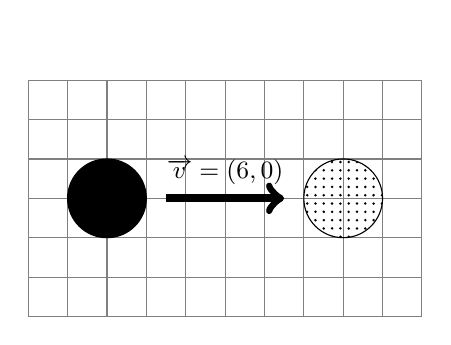
\begin{tikzpicture}[scale=1]
            \draw[step=0.5cm,gray,thin] (-3,-2) grid (2,1);
            \draw[black, fill = black] (-2,-0.5) circle [radius=.5];
            \draw[black, pattern=dots] (1,-0.5) circle [radius=.5];
            \draw[thick, black, ->, line width=1mm] (-1.25,-0.5) -- node[above]{\small$\overrightarrow{v} = (6,0)$} (0.25,-0.5);
            \draw[thick, white, ->, line width=0.001mm] (-1.25,1.1) -- node[above]{\small$\overrightarrow{v} = (6,0)$} (-2.75,1.1);
            \end{tikzpicture}
            \subcaption{Detection (Tracking)}
        \end{minipage}
        \begin{minipage}{.45\textwidth}\centering
            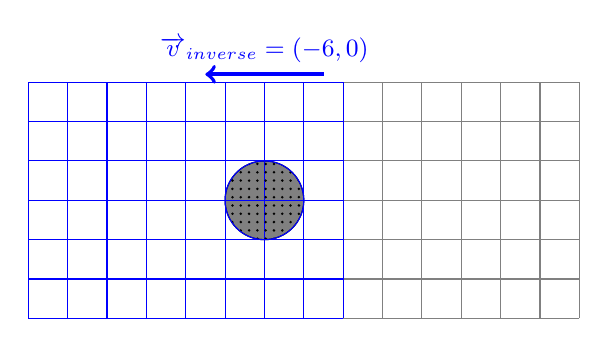
\begin{tikzpicture}[scale=1]
            \draw[step=0.5cm,gray,thin] (-3,-2) grid (2,1);
            \draw[black, fill = gray] (-2,-0.5) circle [radius=.5];
            \draw[thick, blue, ->, line width=0.5mm] (-1.25,1.1) -- node[above]{\small$\overrightarrow{v}_{inverse} = (-6,0)$} (-2.75,1.1);

            \draw[step=0.5cm,blue,thin] (-5,-2) grid (-1,1);
            \draw[blue, pattern=dots] (-2,-0.5) circle [radius=.5];


            \end{tikzpicture}
            \subcaption{Inverse}
        \end{minipage}
        \caption{Translational compensation}
        \label{fig:motionmodel:trans}
    \end{figure}

        \begin{figure}\centering
            \begin{minipage}{.4\textwidth}\centering
                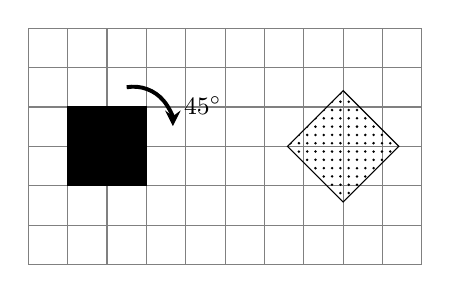
\begin{tikzpicture}[scale=1]
                \draw[step=0.5cm,gray,thin] (-3,-2) grid (2,1);

                \draw[black, fill = black]  (-2.5,0) rectangle (-1.5,-1);
                \draw[black, pattern=dots,rotate around={45:(1,-0.5)}] (0.5,0) rectangle (1.5,-1);
                % \draw[thick, black, ->, line width=1mm] (-1.25,-0.5) -- (0.15,-0.5);
                \draw[-stealth,  black, line width=0.5mm] (-1.75,0.25) arc  (100:0:0.5)node[above right]{\small$45^\circ$};
                \end{tikzpicture}
                \subcaption{Detection (Tracking)}
            \end{minipage}
            \begin{minipage}{.58\textwidth}\centering
                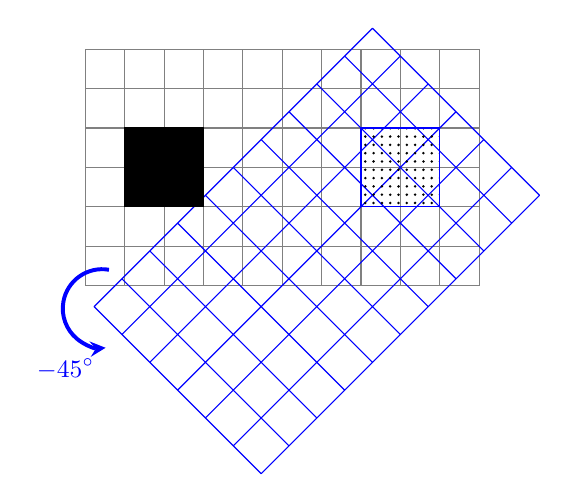
\begin{tikzpicture}[scale=1]
                \draw[step=0.5cm,gray,thin] (-3,-2) grid (2,1);
                \draw[step=0.5cm,blue,rotate around={45:(1,-0.5)},thin] (-3,-2) grid (2,1);

                \draw[black, fill = black]  (-2.5,0) rectangle (-1.5,-1);
                \draw[blue, pattern=dots,] (0.5,0) rectangle (1.5,-1);
                % \draw[thick, black, ->, line width=1mm] (-1.25,-0.5) -- (0.15,-0.5);
                \draw[-stealth,  blue, line width=0.5mm] (-2.7,-1.8) arc  (80:275:0.5)node[below left]{\small$-45^\circ$};
                \end{tikzpicture}
                \subcaption{Inverse}
            \end{minipage}
            \caption[position=left]{Rotational compensation}
            % {\hspace*{-2em}\caption{Rotationsstabilisierung}}
            \label{fig:motionmodel:rota}
        \end{figure}

The implementation is thanks to OpenCV quite simple. Firstly, each frame is resized to:
\begin{equation*}\centering
    \begin{split}
        (width_{new}, height_{new}) =\\
        &(width_{original} + max(globalDeltaData_x),\\
        &~height_{original} + max(globalDeltaData_y))
    \end{split}
\end{equation*}

The translational and rotational transformations can be seen in \cref{lst:transform}. \texttt{cv::Mat} fullfills the frame concept and only differs in its memory management. One flaw in the current implementation, is that the image is rotated around its center. A better solution would be calculation the middle of all relevant tracking areas and using this point as center for the rotation.

\begin{lstlisting}[caption={Frame transformations},label=lst:transform]
void positionShift(cv::Mat &image, frameDeltaVector dv) {
// Perform position shift
cv::Mat trans_mat = (cv::Mat_<double>(2, 3) << 1, 0,
                     dv.deltaPosition.x, 0,
                     1, dv.deltaPosition.y);
cv::warpAffine(image, image, trans_mat, image.size());
}
void rotate(cv::Mat &image, frameDeltaVector dv) {
// Perform rotation
cv::Point2f center((image.cols - 1) / 2.0,
                   (image.rows - 1) / 2.0);
cv::Mat rot = cv::getRotationMatrix2D(center,
                                    dv.deltaAngle, 1.0);

cv::warpAffine(image, image, rot, image.size());
}
\end{lstlisting}

\subsection{Reframing}

\section{Results and future work}




%
% \begin{landscape}
%     % \section{System diagram}
%     \begin{figure}[h!]
%         % \centered\vspace{-4.5cm}\vspace{-4.5cm}
%         \small\centering\vspace{-0.5cm}
%         
\begin{figure}[h!]
% \centered\vspace{-4.5cm}\vspace{-4.5cm}
\small\centering\vspace{-0.5cm}
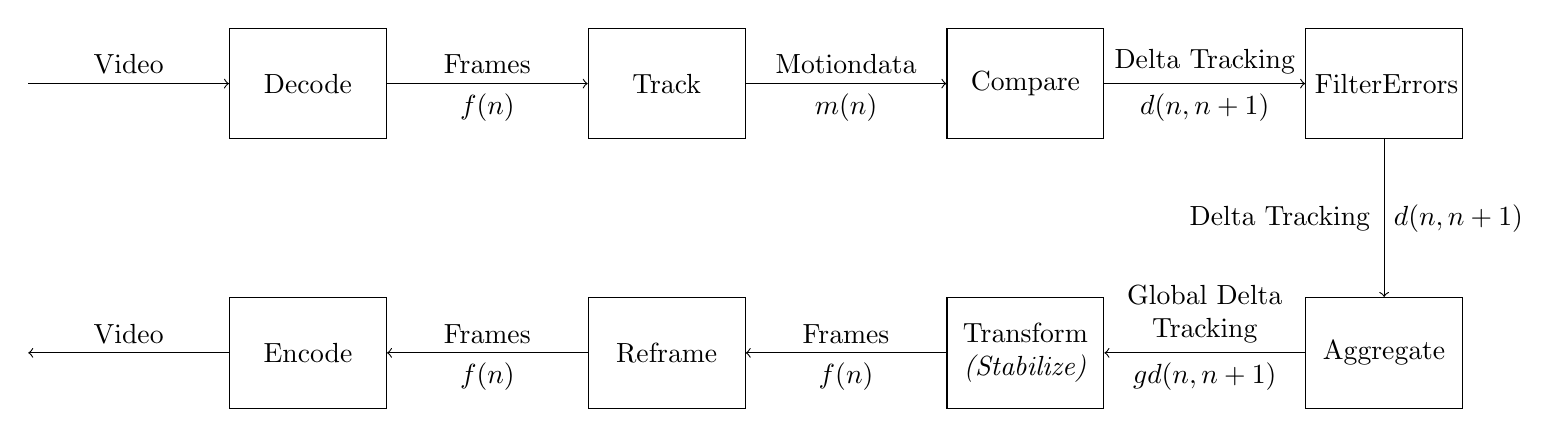
\begin{tikzpicture}[node distance=2cm and 2.55cm,auto]\centering
    \node [input, name=input] {};
    \node [block, right= of input] (pre1) {Decode};
    \node [block, right= of pre1] (analysis1) {Track};
    \node [block, right= of analysis1] (analysis2) {Compare};
    \node [block, right= of analysis2] (analysis3) {FilterErrors};
    \node [block, below= of analysis3] (analysis4) {Aggregate};
    \node [block, left= of analysis4] (stabi) {Transform \textit{(Stabilize)}};
    \node [block, left= of stabi] (post1) {Reframe};
    \node [block, left= of post1] (post2) {Encode};
    \node [input, left=of post2] (output) {t};

    % \node [storage, below right=0.5cm and 0.7cm of analysis] (analysisstorage) {DB};

     \draw[->](input) -- node {Video}(pre1);
     \draw[->](pre1) -- node[label] {Frames} node[below]{$f(n)$}(analysis1);
     \draw[->](analysis1) -- node[label]{Motiondata} node[below]{$m(n)$}(analysis2);
     \draw[->](analysis2) -- node[label]{Delta Tracking} node[below]{$d(n, n+1)$}(analysis3);
     \draw[->](analysis3) -- node[label,left]{Delta Tracking} node[right]{$d(n, n+1)$}(analysis4);
     \draw[->](analysis4) -- node[label,above]{Global Delta Tracking} node[below]{$gd(n, n+1)$}(stabi);
     \draw[->](stabi) -- node[label,above]{Frames} node[below]{$f(n)$}(post1);
     \draw[->](post1) -- node[label,above]{Frames} node[below]{$f(n)$}(post2);


     \draw[->](post2) -- node[above]{Video}(output);
\end{tikzpicture}
\caption{High-level system diagram}
\end{figure}

\tikzstyle{wideblock} = [rectangle, draw, text width=7em, text centered,  minimum height=4em]
\begin{figure}\centering\vspace{-4.5cm}
    \tcbox[enhanced, sharp corners, boxsep=1mm, boxrule=1mm,colframe=gray!10!white,
        colback=white,
        borderline={2pt}{-1pt}{gray,dotted}]
        {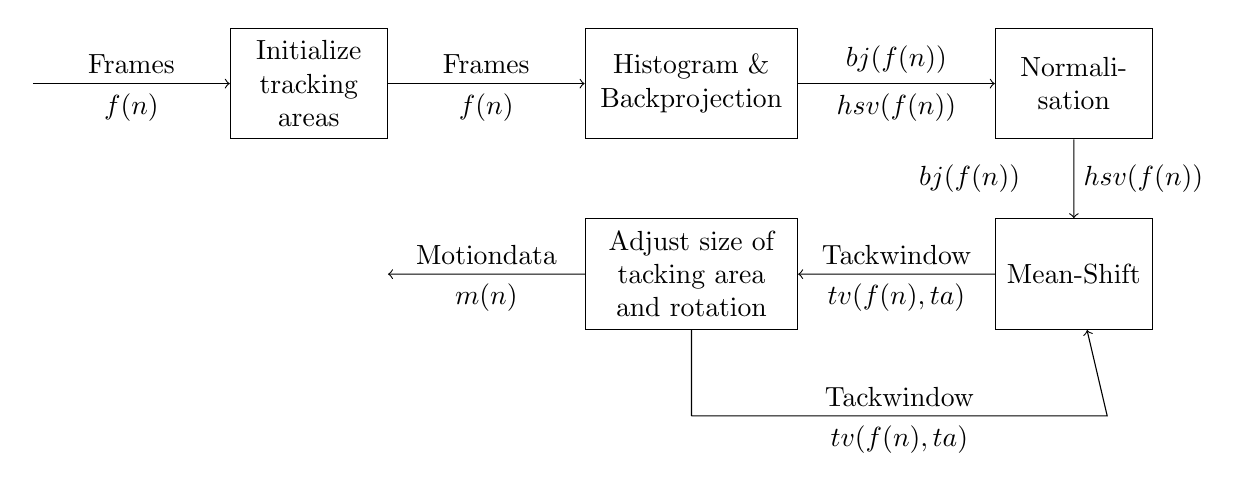
\begin{tikzpicture}[scale=0.6,node distance=1cm and 2.5cm,auto]
            \node [input, name=input] {};
            \node [block, right= of input] (pre1) {Initialize tracking areas};
            \node [wideblock, right= of pre1] (pre2) {Histogram \& Backprojection};
            \node [block, right= of pre2] (pre3) {Normali-sation};
            \node [block, below= of pre3] (pre4) {Mean-Shift};
            \node [wideblock, left= of pre4] (pre5) {Adjust size of tacking area and rotation};
            \node [input, left=of pre5] (output) {t};

            \draw[->](input) -- node[label]{Frames}node[below]{$f(n)$}(pre1);
            \draw[->](pre1) -- node[label]{Frames}node[below]{$f(n)$}(pre2);


            \draw[->](pre2) -- node[label]{$bj(f(n))$}node[below]{$hsv(f(n))$}(pre3);

            \draw[->](pre3) -- node[label, left]{$bj(f(n))$}node[right]{$hsv(f(n))$}(pre4);


            \draw[->](pre4) -- node[label, above]{Tackwindow}node[below]{$tv(f(n), ta)$}(pre5);
            \draw[->](pre5)  |- ++(0,-3cm) --node[label, above]{Tackwindow}node[below]{$tv(f(n), ta)$} ++(8.8cm,0) -- (pre4);


            \draw[->](pre5) -- node[label, above]{Motiondata}node[below]{$m(n)$}(output);
        \end{tikzpicture}
        }
    \caption{Track: CamShift algorithms}
    \label{fig:motionmodels}
\end{figure}

%         \caption{High-level system diagram}
%     \end{figure}
%     \begin{figure}\centering\vspace{-4.5cm}
%         
    \tcbox[enhanced, sharp corners, boxsep=1mm, boxrule=1mm,colframe=gray!10!white,
        colback=white,
        borderline={2pt}{-1pt}{gray,dotted}]
        {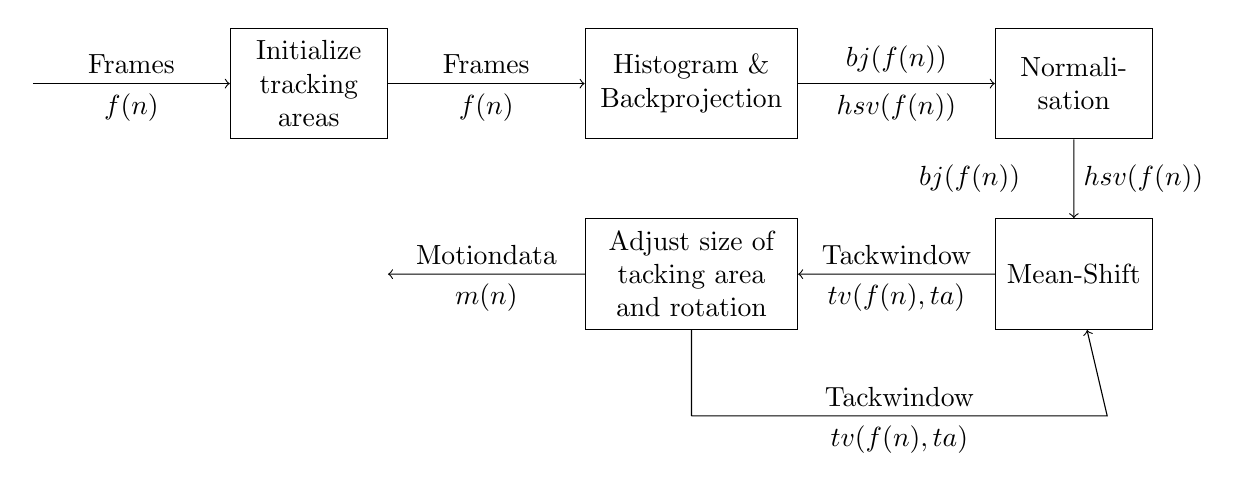
\begin{tikzpicture}[scale=0.6,node distance=1cm and 2.5cm,auto]
            \node [input, name=input] {};
            \node [block, right= of input] (pre1) {Initialize tracking areas};
            \node [wideblock, right= of pre1] (pre2) {Histogram \& Backprojection};
            \node [block, right= of pre2] (pre3) {Normali-sation};
            \node [block, below= of pre3] (pre4) {Mean-Shift};
            \node [wideblock, left= of pre4] (pre5) {Adjust size of tacking area and rotation};
            \node [input, left=of pre5] (output) {t};

            \draw[->](input) -- node[label]{Frames}node[below]{$f(n)$}(pre1);
            \draw[->](pre1) -- node[label]{Frames}node[below]{$f(n)$}(pre2);


            \draw[->](pre2) -- node[label]{$bj(f(n))$}node[below]{$hsv(f(n))$}(pre3);

            \draw[->](pre3) -- node[label, left]{$bj(f(n))$}node[right]{$hsv(f(n))$}(pre4);


            \draw[->](pre4) -- node[label, above]{Tackwindow}node[below]{$tv(f(n), ta)$}(pre5);
            \draw[->](pre5)  |- ++(0,-3cm) --node[label, above]{Tackwindow}node[below]{$tv(f(n), ta)$} ++(8.8cm,0) -- (pre4);


            \draw[->](pre5) -- node[label, above]{Motiondata}node[below]{$m(n)$}(output);
        \end{tikzpicture}
        }

%         \caption{Track: CamShift algorithms}
%         \label{fig:motionmodels}
%     \end{figure}
%     % 
\begin{figure}[h!]
% \centered\vspace{-4.5cm}\vspace{-4.5cm}
\small\centering\vspace{-0.5cm}
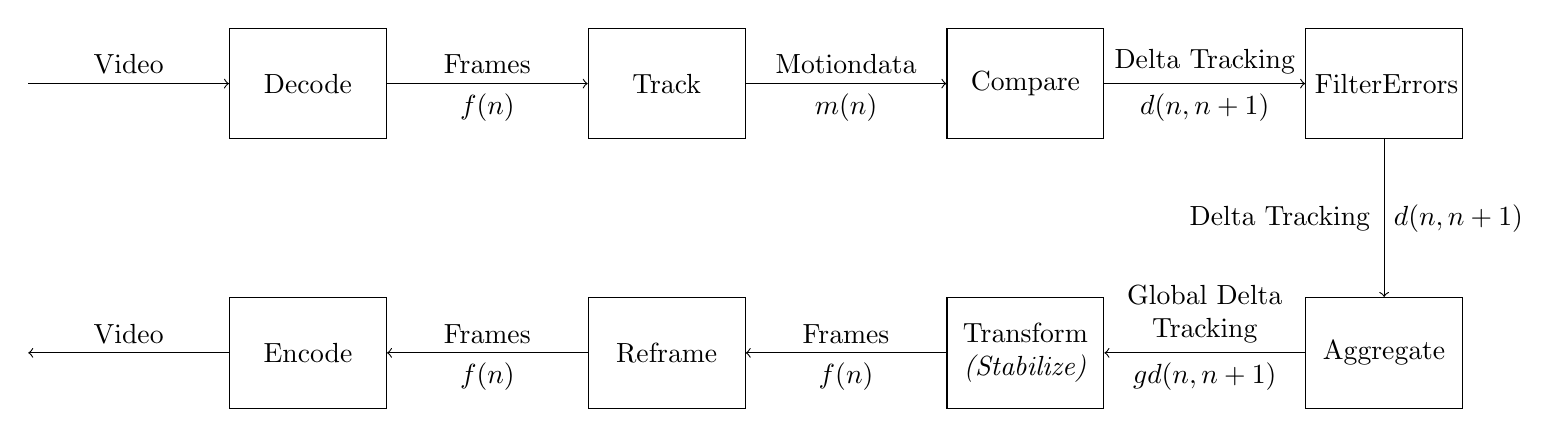
\begin{tikzpicture}[node distance=2cm and 2.55cm,auto]\centering
    \node [input, name=input] {};
    \node [block, right= of input] (pre1) {Decode};
    \node [block, right= of pre1] (analysis1) {Track};
    \node [block, right= of analysis1] (analysis2) {Compare};
    \node [block, right= of analysis2] (analysis3) {FilterErrors};
    \node [block, below= of analysis3] (analysis4) {Aggregate};
    \node [block, left= of analysis4] (stabi) {Transform \textit{(Stabilize)}};
    \node [block, left= of stabi] (post1) {Reframe};
    \node [block, left= of post1] (post2) {Encode};
    \node [input, left=of post2] (output) {t};

    % \node [storage, below right=0.5cm and 0.7cm of analysis] (analysisstorage) {DB};

     \draw[->](input) -- node {Video}(pre1);
     \draw[->](pre1) -- node[label] {Frames} node[below]{$f(n)$}(analysis1);
     \draw[->](analysis1) -- node[label]{Motiondata} node[below]{$m(n)$}(analysis2);
     \draw[->](analysis2) -- node[label]{Delta Tracking} node[below]{$d(n, n+1)$}(analysis3);
     \draw[->](analysis3) -- node[label,left]{Delta Tracking} node[right]{$d(n, n+1)$}(analysis4);
     \draw[->](analysis4) -- node[label,above]{Global Delta Tracking} node[below]{$gd(n, n+1)$}(stabi);
     \draw[->](stabi) -- node[label,above]{Frames} node[below]{$f(n)$}(post1);
     \draw[->](post1) -- node[label,above]{Frames} node[below]{$f(n)$}(post2);


     \draw[->](post2) -- node[above]{Video}(output);
\end{tikzpicture}
\caption{High-level system diagram}
\end{figure}

\tikzstyle{wideblock} = [rectangle, draw, text width=7em, text centered,  minimum height=4em]
\begin{figure}\centering\vspace{-4.5cm}
    \tcbox[enhanced, sharp corners, boxsep=1mm, boxrule=1mm,colframe=gray!10!white,
        colback=white,
        borderline={2pt}{-1pt}{gray,dotted}]
        {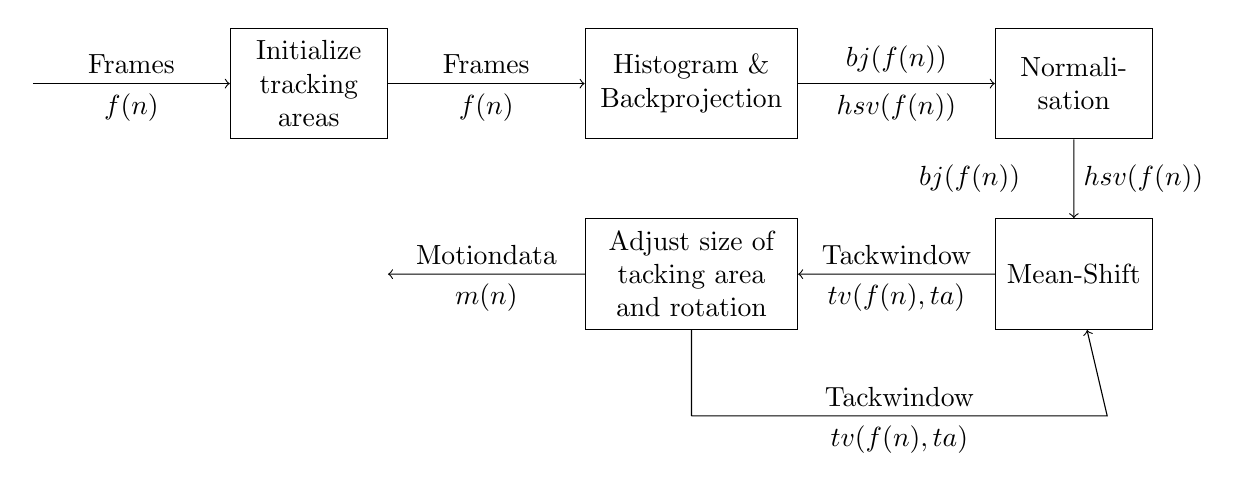
\begin{tikzpicture}[scale=0.6,node distance=1cm and 2.5cm,auto]
            \node [input, name=input] {};
            \node [block, right= of input] (pre1) {Initialize tracking areas};
            \node [wideblock, right= of pre1] (pre2) {Histogram \& Backprojection};
            \node [block, right= of pre2] (pre3) {Normali-sation};
            \node [block, below= of pre3] (pre4) {Mean-Shift};
            \node [wideblock, left= of pre4] (pre5) {Adjust size of tacking area and rotation};
            \node [input, left=of pre5] (output) {t};

            \draw[->](input) -- node[label]{Frames}node[below]{$f(n)$}(pre1);
            \draw[->](pre1) -- node[label]{Frames}node[below]{$f(n)$}(pre2);


            \draw[->](pre2) -- node[label]{$bj(f(n))$}node[below]{$hsv(f(n))$}(pre3);

            \draw[->](pre3) -- node[label, left]{$bj(f(n))$}node[right]{$hsv(f(n))$}(pre4);


            \draw[->](pre4) -- node[label, above]{Tackwindow}node[below]{$tv(f(n), ta)$}(pre5);
            \draw[->](pre5)  |- ++(0,-3cm) --node[label, above]{Tackwindow}node[below]{$tv(f(n), ta)$} ++(8.8cm,0) -- (pre4);


            \draw[->](pre5) -- node[label, above]{Motiondata}node[below]{$m(n)$}(output);
        \end{tikzpicture}
        }
    \caption{Track: CamShift algorithms}
    \label{fig:motionmodels}
\end{figure}

% \end{landscape}
% \section{Coding Concepts}
% \begin{description}
    \item[preprocessing]
    \begin{table}[ht]
    \begin{tabular}{@{}llll@{}}
    \toprule
    \textbf{Expression} & \textbf{Return} & \textbf{Equivalent expression} & \textbf{Notes} \\ \midrule
       &                 &                                &                \\
                    &                 &                                &                \\ \bottomrule
    \end{tabular}
    \end{table}
\end{description}



\printbibliography\cleardoublepage

\end{document}
